\documentclass[aspectratio=169]{beamer}

\usetheme{Warsaw}
\usecolortheme{default}
\usefonttheme{structurebold}

\usepackage[utf8]{inputenc}
\usepackage[brazil]{babel}
\usepackage{minted}

\beamertemplatenavigationsymbolsempty

\title{Exploiting de Binários}
\author{Thiago Luiz Cavalcante Peixoto}
\institute{Universidade Federal de Alagoas
	    \par
	    Instituto de Computação}
\date{\today}

\begin{document}

% Apresentação
\begin{frame}
	\titlepage
\end{frame}

% Sumário
\begin{frame}{Sumário}
	\tableofcontents
\end{frame}

% Section: Revisão
\section{Revisão}
% Subsection: Arquitetura de Computadores
\subsection{Arquitetura de Computadores}
% A Arquitetura de Von Neumann
\begin{frame}{\subsecname}
A Arquitetura de Von Neumann
\begin{figure}
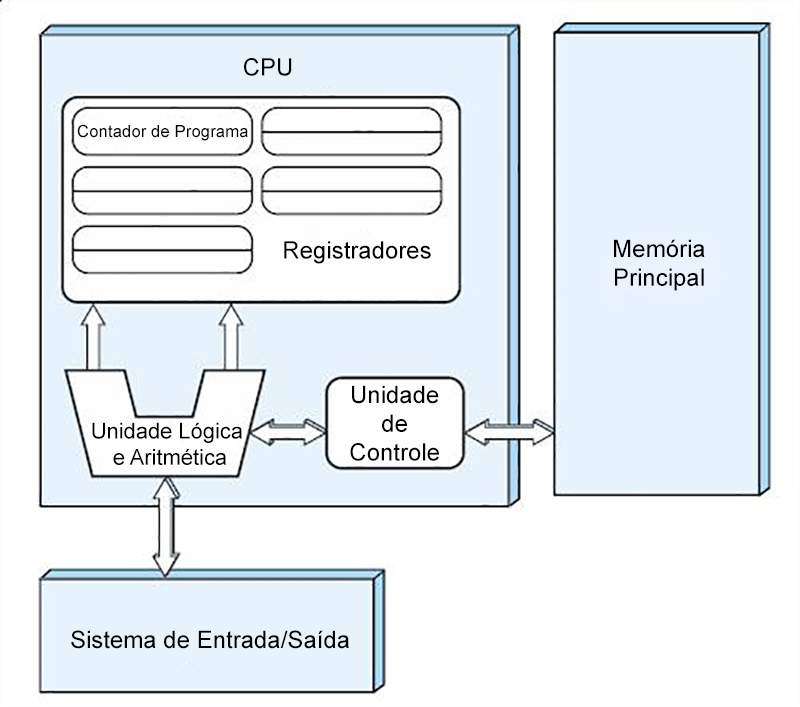
\includegraphics[scale=0.23]{images/Von_Neumann.png}
\end{figure}
\end{frame}

% O Conceito de Abstração
\begin{frame}[fragile]{\subsecname}
O Conceito de Abstração
\begin{columns}
	\begin{column}{0.5\textwidth}
	\begin{figure}
	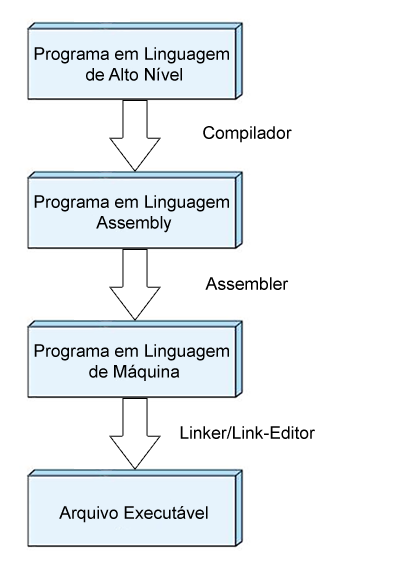
\includegraphics[scale=0.27]{images/Abstracao.png}
	\end{figure}
	\end{column}
	\begin{column}{0.5\textwidth}
		\begin{minted}{c}
int temp = *a;
*a = *b;
*b = temp;
		\end{minted}
		\begin{minted}{asm}
mov eax,DWORD PTR [rdi]
mov edx,DWORD PTR [rsi]
mov DWORD PTR [rdi],edx
mov DWORD PTR [rsi],eax
		\end{minted}
8B 07 8B 16 89 17 89 06
	\end{column}
\end{columns}
\end{frame}

% Subsection: Sistemas Operacionais
\subsection{Sistemas Operacionais}
% Chamadas de Sistema
\begin{frame}{\subsecname}
\begin{block}{Chamadas de Sistema}
Lorem ipsum dolor sit amet, consectetur adipisicing elit, sed do eiusmod tempor incididunt ut labore et dolore magna aliqua.
\end{block}
\begin{figure}
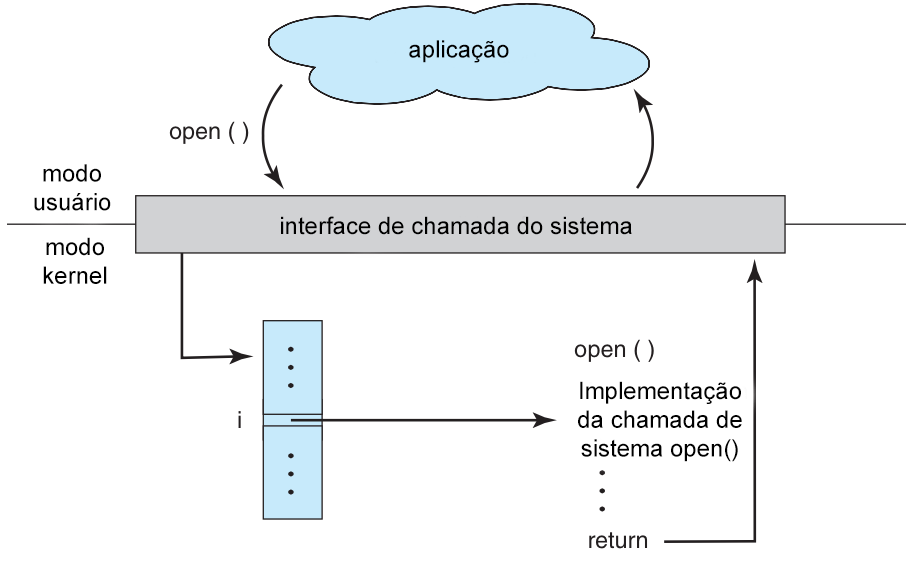
\includegraphics[scale=0.20]{images/Chamadas_Sistema.png}
\end{figure}
\end{frame}

% Subsection: Segmentação de Memória
\subsection{Segmentação de Memória}
% Segmentação de Memória
\begin{frame}{\subsecname}
A memória de um programa compilado é dividida em 5 segmentos:
		\begin{itemize}
			\item \textbf{text}
			\begin{itemize}
				\item[] Instruções de linguagem de máquina.
			\end{itemize}
			\item \textbf{data}
			\begin{itemize}
				\item[] Variáveis globais e estáticas inicializadas.
			\end{itemize}
			\item \textbf{bss}
			\begin{itemize}
				\item[] Variáveis globais e estáticas não inicializadas.
			\end{itemize}
			\item \textbf{heap}
			\begin{itemize}
				\item[] Blocos de memória alocados dinamicamente.
			\end{itemize}
			\item \textbf{stack}
			\begin{itemize}
				\item[] Variáveis locais de uma função e contexto durante chamadas de função.
			\end{itemize}
		\end{itemize}
\end{frame}

% Segmentação de Memória
\begin{frame}{\subsecname}
\begin{figure}
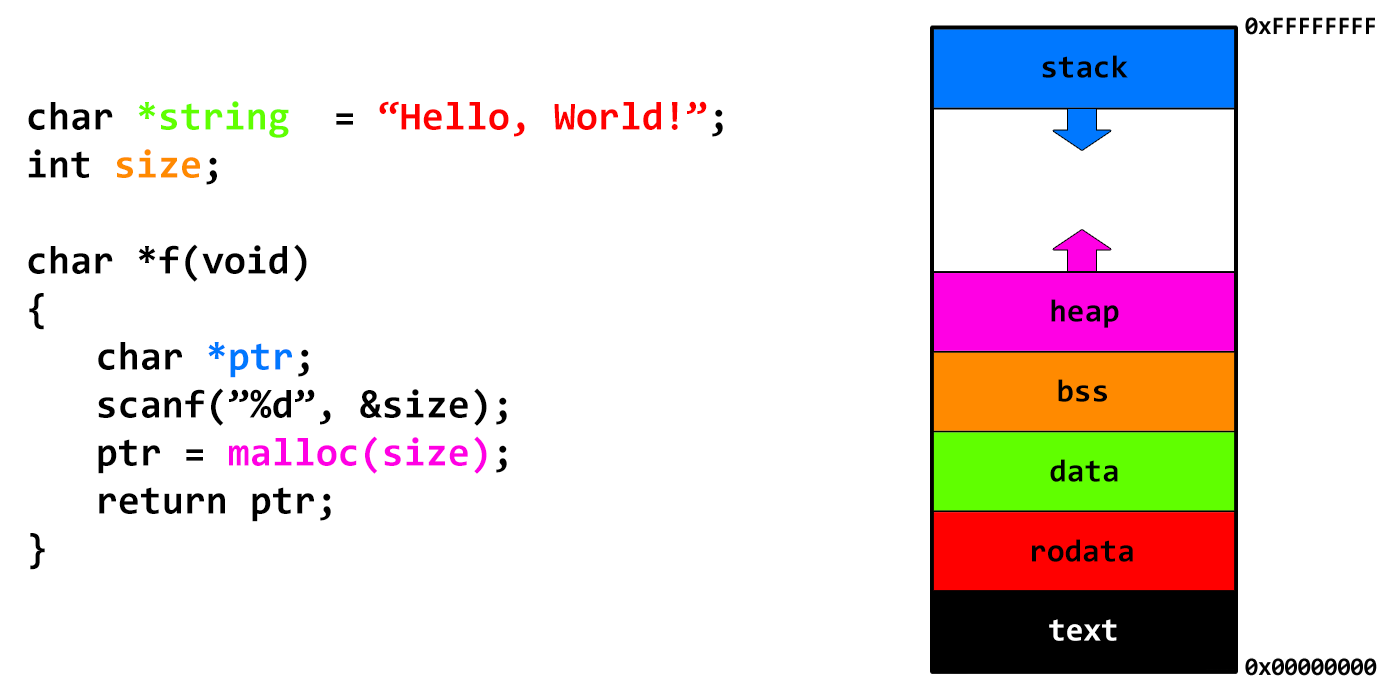
\includegraphics[scale=0.30]{images/Codigo_Segmentos.png}
\end{figure}
\end{frame}

% Segmentação de Memória
\begin{frame}[fragile]{\subsecname}
\begin{columns}
	\begin{column}{0.5\textwidth}
		\begin{minted}{c}
#include <stdlib.h>

void main(void)
{
	exit(10);
}
		\end{minted}
	\end{column}
	\begin{column}{0.5\textwidth}
		\begin{minted}{asm}
section .text
global _start
_start:
        mov rax, [sys_exit]
        mov rdi, [ret_value]
        syscall
section .data
ret_value:  dq 0x0A
sys_exit:   dq 0x3C
		\end{minted}
	\end{column}
\end{columns}
\end{frame}

\section{Arquitetura Intel}
% Arquitetura Intel
\begin{frame}{\secname}
\end{frame}

%Subsection: Registradores de Uso Geral
\subsection{Registradores de Uso Geral}
\begin{frame}{\subsecname}
\end{frame}

%Subsection: Instruções
\subsection{Instruções}
\subsubsection{Avulsas}
% Avulsas
\begin{frame}[fragile]{\subsubsecname}
\begin{columns}
	\begin{column}{0.5\textwidth}
	\begin{block}{NOP}
		\begin{itemize}
			\item Incrementa o registrador EIP para apontar para a próxima instrução;
			\item Alias para \textbf{xchg eax, eax};
			\item Formato da instrução:
			\begin{itemize}
				\item[] nop
			\end{itemize}
		\end{itemize}
	\end{block}
	\end{column}
	\begin{column}{0.5\textwidth}
		\begin{minted}{asm}
section .text
global _start
_start:
	nop
	mov rax, [sys_exit]
	mov rdi, [ret_value]
	syscall
section .data
ret_value:  dq 0x0A
sys_exit:   dq 0x3C
		\end{minted}
	\end{column}
\end{columns}
\end{frame}

\subsubsection{Movimentação de Dados}
% Slide 12
\begin{frame}[fragile]{\subsubsecname}
\begin{columns}
	\begin{column}{0.5\textwidth}
	\begin{block}{MOV}
		\begin{itemize}
			\item Movimentação de dados, no formato \textbf{mov destino, fonte}; 
			\item Formato da instrução:
			\begin{itemize}
				\item[] mov reg/mem, imm
				\item[] mov reg/mem, reg
				\item[] mov reg, mem
			\end{itemize}
		\end{itemize}
	\end{block}
	\end{column}
	\begin{column}{0.5\textwidth}
		\begin{minted}{asm}
section .text
global _start
_start:
	mov eax, [array]
	mov dword [array + 4], 0x0E 
	mov ebx, 2
	mov eax, [ebx * 4 + array]
	mov edx, array
	mov eax, [edx + ebx * 4 + 4]
	mov rax, 0x3C
	xor rdi, rdi
	syscall
section .data
array: dd 0x0A, 0x0B, 0x0C, 0x0D
		\end{minted}
	\end{column}
\end{columns}
\end{frame}

% Slide 13
\begin{frame}[fragile]{\subsubsecname}
\begin{columns}
	\begin{column}{0.5\textwidth}
	\begin{block}{XCHG}
		\begin{itemize}
			\item Troca de dados entre dois operandos, no formato \textbf{xchg op1, op2};
			\item O processador usa o sinal LOCK quando um dos operandos estiver na memória;
			\item Formato da instrução:
			\begin{itemize}
				\item[] xchg reg/mem, reg
				\item[] xchg reg, mem
			\end{itemize}
		\end{itemize}
	\end{block}
	\end{column}
	\begin{column}{0.5\textwidth}
		\begin{minted}{asm}
section .text
global _start
_start:
	mov eax, 0x09
	mov ebx, 0x01
	xchg eax, ebx
	xchg ebx, [num]
	mov rax, 0x3C
	xor rdi, rdi
	syscall
section .data
num: dd 0x0A
		\end{minted}
	\end{column}
\end{columns}
\end{frame}

\subsubsection{Aritméticas}
% Slide 14
\begin{frame}[fragile]{\subsubsecname}
\begin{columns}
	\begin{column}{0.5\textwidth}
	\begin{block}{ADD}
		\begin{itemize}
			\item Adição de dois valores inteiros, no formato \textbf{add destino, fonte};
			\item Observar a CARRY FLAG na soma de inteiros sem sinal e a OVERFLOW FLAG na soma de inteiros com sinal;
			\item Formato da instrução:
			\begin{itemize}
				\item[] add reg/mem, imm
				\item[] add reg/mem, reg
				\item[] add reg, mem
			\end{itemize}
		\end{itemize}
	\end{block}
	\end{column}
	\begin{column}{0.5\textwidth}
		\begin{minted}{asm}
section .text
global _start
_start:
	mov ecx, 0x01
	mov ebx, 0x02
	add ebx, ecx
	add ebx, [num]
	add [num], ebx
	mov rax, 0x3C
	xor rdi, rdi
	syscall
section .data
num: dd 0x07
		\end{minted}
	\end{column}
\end{columns}
\end{frame}

% Slide 15
\begin{frame}[fragile]{\subsubsecname}
\begin{columns}
	\begin{column}{0.5\textwidth}
	\begin{block}{ADC}
		\begin{itemize}
			\item Movimentação de dados no seguinte formato: \textbf{mov destino, fonte}; 
			\item Formato:
			\begin{itemize}
				\item[] mov reg/mem, imm
				\item[] mov reg/mem, reg
				\item[] mov reg, mem
			\end{itemize}
		\end{itemize}
	\end{block}
	\end{column}
	\begin{column}{0.5\textwidth}
		\begin{minted}{asm}
section .text
global _start
_start:
	mov al, 0xFF
	mov ah, 0x00
	mov bl, 0xFF
	mov bh, 0x00
	add al, bl
	adc ah, bh
	mov rax, 0x3C
	xor rdi, rdi
	syscall
		\end{minted}
	\end{column}
\end{columns}
\end{frame}

% Slide 16
\begin{frame}[fragile]{\subsubsecname}
\begin{columns}
	\begin{column}{0.5\textwidth}
	\begin{block}{SUB}
		\begin{itemize}
			\item Movimentação de dados no seguinte formato: \textbf{mov destino, fonte}; 
			\item Formato:
			\begin{itemize}
				\item[] mov reg/mem, imm
				\item[] mov reg/mem, reg
				\item[] mov reg, mem
			\end{itemize}
		\end{itemize}
	\end{block}
	\end{column}
	\begin{column}{0.5\textwidth}
		\begin{minted}{asm}
section .text
global _start
_start:
	mov ecx, 0x01
	mov ebx, 0x0F
	sub ebx, ecx
	sub ebx, [num]
	sub ebx, 0x01
	sub [num], ebx
	mov rax, 0x3C
	xor rdi, rdi
	syscall
section .data
num: dd 0x04
		\end{minted}
	\end{column}
\end{columns}
\end{frame}

% Slide 17
\begin{frame}[fragile]{\subsubsecname}
\begin{columns}
	\begin{column}{0.5\textwidth}
	\begin{block}{SBB}
		\begin{itemize}
			\item Movimentação de dados no seguinte formato: \textbf{mov destino, fonte}; 
			\item Formato:
			\begin{itemize}
				\item[] mov reg/mem, imm
				\item[] mov reg/mem, reg
				\item[] mov reg, mem
			\end{itemize}
		\end{itemize}
	\end{block}
	\end{column}
	\begin{column}{0.5\textwidth}
		\begin{minted}{asm}
section .text
global _start
_start:
	mov al, 0x7F
	mov ah, 0x00
	mov bl, 0xFF
	mov bh, 0x00
	sub al, bl
	sbb ah, bh
	mov rax, 0x3C
	xor rdi, rdi
	syscall
		\end{minted}
	\end{column}
\end{columns}
\end{frame}

% Slide 18
\begin{frame}[fragile]{\subsubsecname}
\begin{columns}
	\begin{column}{0.5\textwidth}
	\begin{block}{INC}
		\begin{itemize}
			\item Incrementa o conteúdo do operando em 1, no formato \textbf{inc op}; 
			\item Não afeta a CARRY FLAG;
			\item Formato da instrução:
			\begin{itemize}
				\item[] inc reg/mem
			\end{itemize}
		\end{itemize}
	\end{block}
	\end{column}
	\begin{column}{0.5\textwidth}
		\begin{minted}{asm}
section .text
global _start
_start:
	mov ebx, 0x0A
	inc ebx
	inc dword [num]
	mov rax, 0x3c
	xor rdi, rdi
	syscall
section .data
num: dd 0x07
		\end{minted}
	\end{column}
\end{columns}
\end{frame}

% Slide 19
\begin{frame}[fragile]{\subsubsecname}
\begin{columns}
	\begin{column}{0.5\textwidth}
	\begin{block}{DEC}
		\begin{itemize}
			\item Decrementa o conteúdo do operando em 1, no formato \textbf{dec op};
			\item Não afeta a CARRY FLAG;
			\item Formato da instrução:
			\begin{itemize}
				\item[] dec reg/mem
			\end{itemize}
		\end{itemize}
	\end{block}
	\end{column}
	\begin{column}{0.5\textwidth}
		\begin{minted}{asm}
section .text
global _start
_start:
	mov ebx, 0x0A
	dec ebx
	dec dword [num]
	mov rax, 0x3c
	xor rdi, rdi
	syscall
section .data
num: dd 0x07
		\end{minted}
	\end{column}
\end{columns}
\end{frame}

% Slide 20
\begin{frame}[fragile]{\subsubsecname}
\begin{columns}
	\begin{column}{0.5\textwidth}
	\begin{block}{MUL}
		\begin{itemize}
			\item Movimentação de dados no seguinte formato: \textbf{mov destino, fonte}; 
			\item Formato:
			\begin{itemize}
				\item[] mov reg/mem, imm
				\item[] mov reg/mem, reg
				\item[] mov reg, mem
			\end{itemize}
		\end{itemize}
	\end{block}
	\end{column}
	\begin{column}{0.5\textwidth}
		\begin{minted}{asm}
section .text
global _start
_start:
	mov rax, 0x0A
	mov rbx, 0x03
	mul rbx
	mul qword [num]
	mov rax, 0x3C
	xor rdi, rdi
	syscall
section .data
num: dq 0x02
		\end{minted}
	\end{column}
\end{columns}
\end{frame}

% Slide 21
\begin{frame}[fragile]{\subsubsecname}
\begin{columns}
	\begin{column}{0.5\textwidth}
	\begin{block}{IMUL}
		\begin{itemize}
			\item Movimentação de dados no seguinte formato: \textbf{mov destino, fonte}; 
			\item Formato:
			\begin{itemize}
				\item[] mov reg/mem, imm
				\item[] mov reg/mem, reg
				\item[] mov reg, mem
			\end{itemize}
		\end{itemize}
	\end{block}
	\end{column}
	\begin{column}{0.5\textwidth}
		\begin{minted}{asm}
section .text
global _start
_start:
	mov rax, 0x0A
	mov rbx, 0x03
	imul rbx
	imul rax, [num]
	imul rax, rax, 0x02
	mov rax, 0x3C
	xor rdi, rdi
	syscall
section .data
num: dq 0x02
		\end{minted}
	\end{column}
\end{columns}
\end{frame}

% Slide 22
\begin{frame}[fragile]{\subsubsecname}
\begin{columns}
	\begin{column}{0.5\textwidth}
	\begin{block}{DIV}
		\begin{itemize}
			\item Movimentação de dados no seguinte formato: \textbf{mov destino, fonte}; 
			\item Formato:
			\begin{itemize}
				\item[] mov reg/mem, imm
				\item[] mov reg/mem, reg
				\item[] mov reg, mem
			\end{itemize}
		\end{itemize}
	\end{block}
	\end{column}
	\begin{column}{0.5\textwidth}
		\begin{minted}{asm}
section .text
global _start
_start:
	mov eax, 0x64
	mov ebx, 0x04
	mov edx, 0x00
	div ebx
	div dword [num]
	mov rax, 0x3C
	xor rdi, rdi
	syscall
section .data
num: dd 0x05
		\end{minted}
	\end{column}
\end{columns}
\end{frame}

% Slide 23
\begin{frame}[fragile]{\subsubsecname}
\begin{columns}
	\begin{column}{0.5\textwidth}
	\begin{block}{IDIV}
		\begin{itemize}
			\item Movimentação de dados no seguinte formato: \textbf{mov destino, fonte}; 
			\item Formato:
			\begin{itemize}
				\item[] mov reg/mem, imm
				\item[] mov reg/mem, reg
				\item[] mov reg, mem
			\end{itemize}
		\end{itemize}
	\end{block}
	\end{column}
	\begin{column}{0.5\textwidth}
		\begin{minted}{asm}
section .text
global _start
_start:
	mov eax, [num]
	mov ebx, 0x02
	mov edx, 0xFFFFFFFF
	idiv ebx
	mov rax, 0x3C
	xor rdi, rdi
	syscall
section .data
num: dd 0xFFFFFFF8
		\end{minted}
	\end{column}
\end{columns}
\end{frame}

\subsubsection{Deslocamento de Bits}
% Slide 23
\begin{frame}[fragile]{\subsubsecname}
\begin{columns}
	\begin{column}{0.5\textwidth}
	\begin{block}{SHL/SAL}
		\begin{itemize}
			\item Movimentação de dados no seguinte formato: \textbf{mov destino, fonte}; 
			\item Formato:
			\begin{itemize}
				\item[] mov reg/mem, imm
				\item[] mov reg/mem, reg
				\item[] mov reg, mem
			\end{itemize}
		\end{itemize}
	\end{block}
	\end{column}
	\begin{column}{0.5\textwidth}
		\begin{minted}{asm}
section .text
global _start
_start:
	mov al, 0xFF
	shl al, 1
	mov cl, 0x02
	sal al, cl
	mov rax, 0x3C
	xor rdi, rdi
	syscall
		\end{minted}
	\end{column}
\end{columns}
\end{frame}

% Slide 23
\begin{frame}[fragile]{\subsubsecname}
\begin{columns}
	\begin{column}{0.5\textwidth}
	\begin{block}{SHR}
		\begin{itemize}
			\item Movimentação de dados no seguinte formato: \textbf{mov destino, fonte}; 
			\item Formato:
			\begin{itemize}
				\item[] mov reg/mem, imm
				\item[] mov reg/mem, reg
				\item[] mov reg, mem
			\end{itemize}
		\end{itemize}
	\end{block}
	\end{column}
	\begin{column}{0.5\textwidth}
		\begin{minted}{asm}
section .text
global _start
_start:
	mov al, 0x10
	mov cl, 0x03
	shr al, cl
	mov rax, 0x3c
	xor rdi, rdi
	syscall
		\end{minted}
	\end{column}
\end{columns}
\end{frame}

% Slide 23
\begin{frame}[fragile]{\subsubsecname}
\begin{columns}
	\begin{column}{0.5\textwidth}
	\begin{block}{SAR}
		\begin{itemize}
			\item Movimentação de dados no seguinte formato: \textbf{mov destino, fonte}; 
			\item Formato:
			\begin{itemize}
				\item[] mov reg/mem, imm
				\item[] mov reg/mem, reg
				\item[] mov reg, mem
			\end{itemize}
		\end{itemize}
	\end{block}
	\end{column}
	\begin{column}{0.5\textwidth}
		\begin{minted}{asm}
section .text
global _start
_start:
	mov al, 0xF0
	mov cl, 0x03
	sar al, cl
	mov rax, 0x3C
	xor rdi, rdi
	syscall
		\end{minted}
	\end{column}
\end{columns}
\end{frame}

% Slide 23
\begin{frame}[fragile]{\subsubsecname}
\begin{columns}
	\begin{column}{0.5\textwidth}
	\begin{block}{ROR}
		\begin{itemize}
			\item Movimentação de dados no seguinte formato: \textbf{mov destino, fonte}; 
			\item Formato:
			\begin{itemize}
				\item[] mov reg/mem, imm
				\item[] mov reg/mem, reg
				\item[] mov reg, mem
			\end{itemize}
		\end{itemize}
	\end{block}
	\end{column}
	\begin{column}{0.5\textwidth}
		\begin{minted}{asm}
section .text
global _start
_start:
	mov al, 0x8F
	ror al, 0x03
	mov rax, 0x3c
	xor rdi, rdi
	syscall
		\end{minted}
	\end{column}
\end{columns}
\end{frame}

% Slide 23
\begin{frame}[fragile]{\subsubsecname}
\begin{columns}
	\begin{column}{0.5\textwidth}
	\begin{block}{ROL}
		\begin{itemize}
			\item Movimentação de dados no seguinte formato: \textbf{mov destino, fonte}; 
			\item Formato:
			\begin{itemize}
				\item[] mov reg/mem, imm
				\item[] mov reg/mem, reg
				\item[] mov reg, mem
			\end{itemize}
		\end{itemize}
	\end{block}
	\end{column}
	\begin{column}{0.5\textwidth}
		\begin{minted}{asm}
section .text
global _start
_start:
	mov al, 0x8F
	mov cl, 0x03
	rol al, cl
	mov rax, 0x3C
	xor rdi, rdi
	syscall
		\end{minted}
	\end{column}
\end{columns}
\end{frame}

\subsubsection{Lógicas}
% Slide 23
\begin{frame}[fragile]{\subsubsecname}
\begin{columns}
	\begin{column}{0.5\textwidth}
	\begin{block}{NOT}
		\begin{itemize}
			\item NOT bit a bit; 
			\item Formato:
			\begin{itemize}
				\item[] not reg/mem
			\end{itemize}
		\end{itemize}
	\end{block}
	\end{column}
	\begin{column}{0.5\textwidth}
		\begin{minted}{asm}
section .text
global _start
_start:
	mov al, 0x0F
	not al
	mov rax, 0x3C
	xor rdi, rdi
	syscall
		\end{minted}
	\end{column}
\end{columns}
\end{frame}

\begin{frame}[fragile]{\subsubsecname}
\begin{columns}
	\begin{column}{0.5\textwidth}
	\begin{block}{AND}
		\begin{itemize}
			\item AND bit a bit; 
			\item Formato:
			\begin{itemize}
				\item[] and reg/mem, imm
				\item[] and reg/mem, reg
				\item[] and reg, mem
			\end{itemize}
		\end{itemize}
	\end{block}
	\end{column}
	\begin{column}{0.5\textwidth}
		\begin{minted}{asm}
section .text
global _start
_start:
	and dword [num], 0x03
	mov rax, 0x3C
	xor rdi, rdi
	syscall
section .data
num: dd 0x07
		\end{minted}
	\end{column}
\end{columns}
\end{frame}

\begin{frame}[fragile]{\subsubsecname}
\begin{columns}
	\begin{column}{0.5\textwidth}
	\begin{block}{OR}
		\begin{itemize}
			\item OR bit a bit; 
			\item Formato:
			\begin{itemize}
				\item[] or reg/mem, imm
				\item[] or reg/mem, reg
				\item[] or reg, mem
			\end{itemize}
		\end{itemize}
	\end{block}
	\end{column}
	\begin{column}{0.5\textwidth}
		\begin{minted}{asm}
section .text
global _start
_start:
	mov eax, 0x03
	or eax, dword [num]
	mov rax, 0x3C
	xor rdi, rdi
	syscall
section .data
num: dd 0x07
		\end{minted}
	\end{column}
\end{columns}
\end{frame}

\begin{frame}[fragile]{\subsubsecname}
\begin{columns}
	\begin{column}{0.5\textwidth}
	\begin{block}{XOR}
		\begin{itemize}
			\item XOR bit a bit; 
			\item Formato:
			\begin{itemize}
				\item[] xor reg/mem, imm
				\item[] xor reg/mem, reg
				\item[] xor reg, mem
			\end{itemize}
		\end{itemize}
	\end{block}
	\end{column}
	\begin{column}{0.5\textwidth}
		\begin{minted}{asm}
section .text
global _start
_start:
	mov eax, 0x03
	xor eax, dword [num]
	mov rax, 0x3C
	xor rdi, rdi
	syscall
section .data
num: dd 0x07
		\end{minted}
	\end{column}
\end{columns}
\end{frame}

\subsubsection{Controle de Fluxo}
\begin{frame}[fragile]{\subsubsecname}
\begin{columns}
	\begin{column}{0.5\textwidth}
	\begin{block}{JMP}
		\begin{itemize}
			\item Movimentação de dados no seguinte formato: \textbf{mov destino, fonte}; 
			\item Formato:
			\begin{itemize}
				\item[] mov reg/mem, imm
				\item[] mov reg/mem, reg
				\item[] mov reg, mem
			\end{itemize}
		\end{itemize}
	\end{block}
	\end{column}
	\begin{column}{0.5\textwidth}
		\begin{minted}{asm}
section .text
global _start
_start:
	jmp label
	mov rbx, 0x01
	mov rcx, 0x02
label:
	mov rax, 0x3C
	xor rdi, rdi
	syscall
		\end{minted}
	\end{column}
\end{columns}
\end{frame}

\begin{frame}[fragile]{\subsubsecname}
	\begin{block}{J[CONDIÇÃO]}
		\begin{itemize}
			\item Movimentação de dados no seguinte formato: \textbf{mov destino, fonte}; 
			\item Formato:
			\begin{itemize}
				\item[] mov reg/mem, imm
				\item[] mov reg/mem, reg
				\item[] mov reg, mem
			\end{itemize}
		\end{itemize}
	\end{block}
\end{frame}

\begin{frame}[fragile]{\subsubsecname}
\begin{columns}
	\begin{column}{0.5\textwidth}
	\begin{block}{LOOP}
		\begin{itemize}
			\item Movimentação de dados no seguinte formato: \textbf{mov destino, fonte}; 
			\item Formato:
			\begin{itemize}
				\item[] mov reg/mem, imm
				\item[] mov reg/mem, reg
				\item[] mov reg, mem
			\end{itemize}
		\end{itemize}
	\end{block}
	\end{column}
	\begin{column}{0.5\textwidth}
		\begin{minted}{asm}
section .text
global _start
_start:
	mov ecx, 0x0A
label:
	add dword [num], ecx
	loop label
	xor rdi, rdi
	mov rax, 0x3C
	syscall
section .data
num: dd 0x00
		\end{minted}
	\end{column}
\end{columns}
\end{frame}

\begin{frame}[fragile]{\subsubsecname}
\begin{columns}
	\begin{column}{0.5\textwidth}
	\begin{block}{CALL}
		\begin{itemize}
			\item Movimentação de dados no seguinte formato: \textbf{mov destino, fonte}; 
			\item Formato:
			\begin{itemize}
				\item[] mov reg/mem, imm
				\item[] mov reg/mem, reg
				\item[] mov reg, mem
			\end{itemize}
		\end{itemize}
	\end{block}
	\end{column}
	\begin{column}{0.5\textwidth}
		\begin{minted}{asm}
extern printf
section .text
global _start
_start:
	mov rdi, string
	call printf
	xor rdi, rdi
	mov rax, 0x3C
	syscall
section .data
string: db "Uma string!", 0x0A, 0x00
		\end{minted}
	\end{column}
\end{columns}
\end{frame}

\begin{frame}[fragile]{\subsubsecname}
\begin{columns}
	\begin{column}{0.5\textwidth}
	\begin{block}{INT}
		\begin{itemize}
			\item Movimentação de dados no seguinte formato: \textbf{mov destino, fonte}; 
			\item Formato:
			\begin{itemize}
				\item[] mov reg/mem, imm
				\item[] mov reg/mem, reg
				\item[] mov reg, mem
			\end{itemize}
		\end{itemize}
	\end{block}
	\end{column}
	\begin{column}{0.5\textwidth}
		\begin{minted}{asm}
section .text
global _start
_start:
	mov eax, 0x04
	mov ebx, 0x01
	mov ecx, string
	mov edx, tamanho
	int 0x80
	xor ebx, ebx
	mov eax, 0x01
	int 0x80
section .data
string: db "Uma string!", 0x0A
tamanho: equ $ - string
		\end{minted}
	\end{column}
\end{columns}
\end{frame}

\begin{frame}[fragile]{\subsubsecname}
\begin{columns}
	\begin{column}{0.5\textwidth}
	\begin{block}{SYSCALL}
		\begin{itemize}
			\item Movimentação de dados no seguinte formato: \textbf{mov destino, fonte}; 
			\item Formato:
			\begin{itemize}
				\item[] mov reg/mem, imm
				\item[] mov reg/mem, reg
				\item[] mov reg, mem
			\end{itemize}
		\end{itemize}
	\end{block}
	\end{column}
	\begin{column}{0.5\textwidth}
		\begin{minted}{asm}
section .text
global _start
_start:
	mov rax, 0x01
	mov rdi, 0x01
	mov rsi, string
	mov rdx, tamanho
	syscall
	xor rdi, rdi
	mov rax, 0x3C
	syscall
section .data
string: db "Uma string!", 0x0A
tamanho: equ $ - string
		\end{minted}
	\end{column}
\end{columns}
\end{frame}

\end{document}